\chapter{Implementierung des Oszilloskop-Moduls}
\label{ch:osci}

Im weiteren Verlauf meines Praktikums wurde mir die Implementierung des Oszilloskop-Moduls zu 
teil, welches für die Ansteuerung mehrerer Oszilloskope zuständig sein soll. Um dies zu testen 
hat uns der Kunde Diehl Aviation ein LeCroy LC334AM 500MHz Oszilloskop zur Verfügung gestellt, 
welches man in Abbildung \ref{fig:lc334am} betrachten kann.  

\begin{figure}[H]
	\centering
	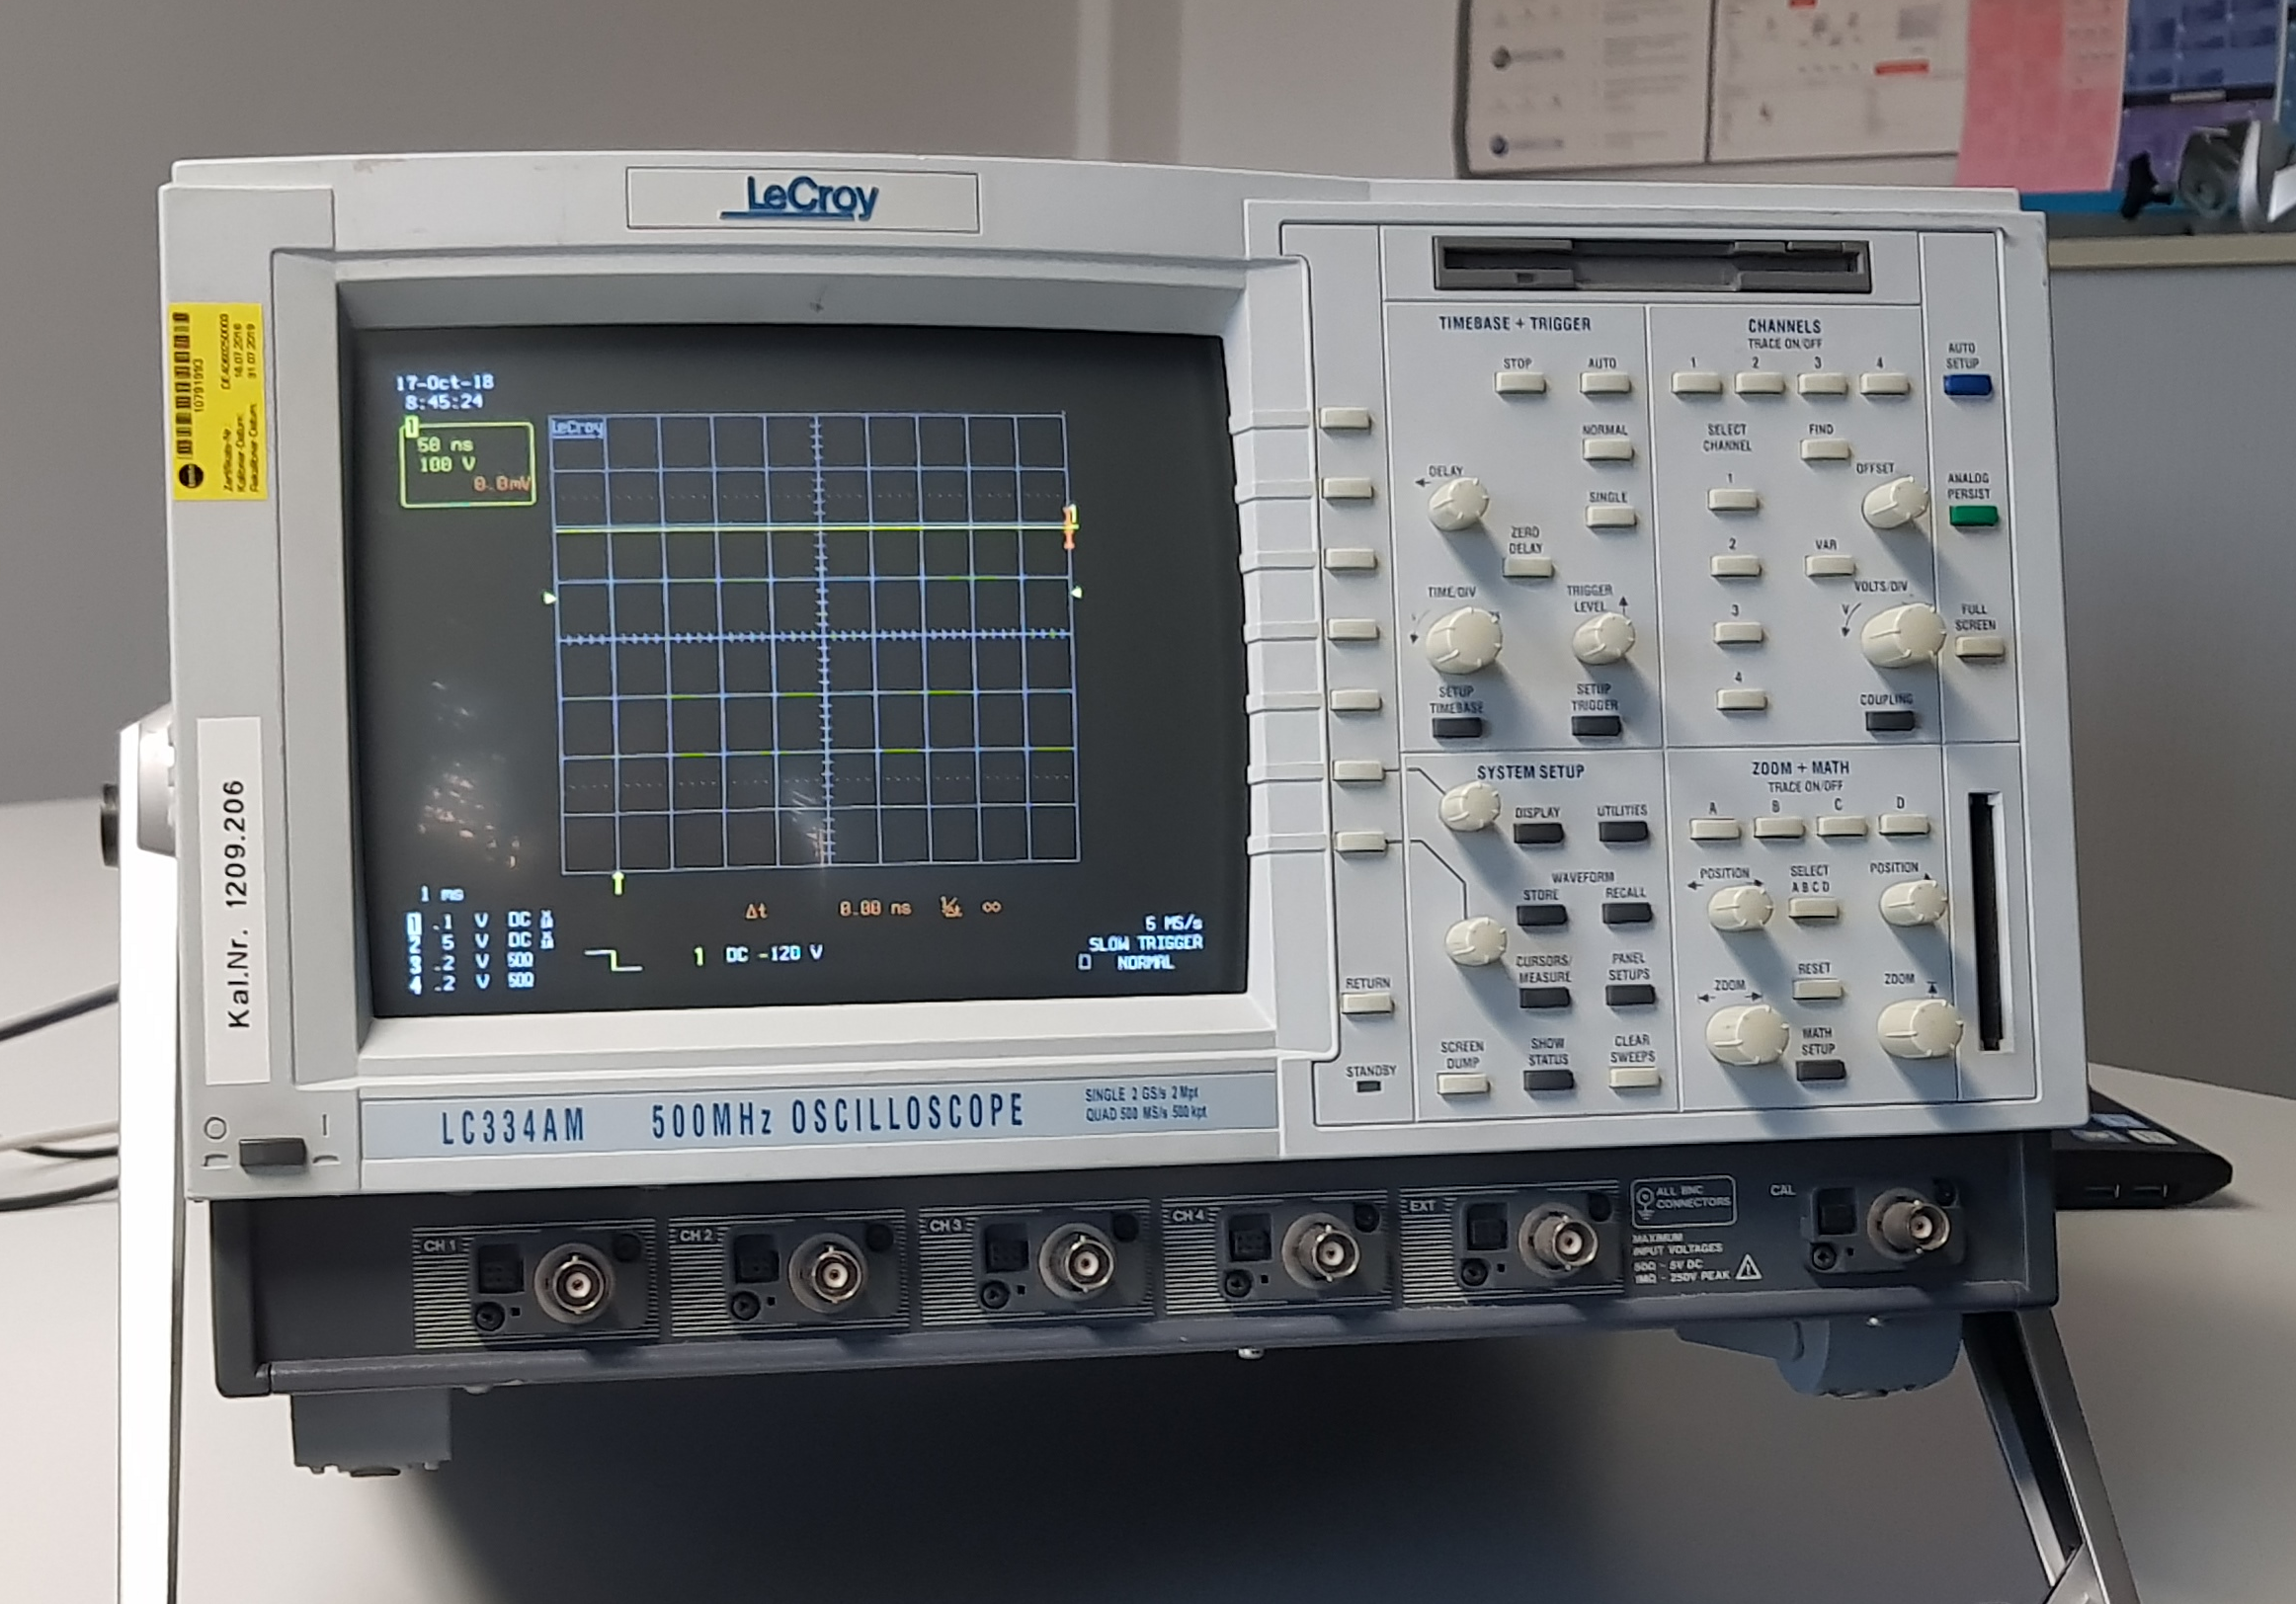
\includegraphics[width=0.75\textwidth, height=0.5\textwidth]{graphics/Programmed_Oscilloscope.png}
	\caption{Lecroy LC334AM 500MHz}
	\label{fig:lc334am}
\end{figure}

\section{Das LeCroy LC334AM 500MHz Oszilloskop}
\label{sec:lc334am}

Das LC334AM 500MHz Oszilloskop von LeCroy\footnote{\url{https://teledynelecroy.com/}} ist dato 
schon ein etwas älteres Gerät, welches über eine \ac{gpib} Schnittstelle und eine \ac{rs232} 
Schnittstelle zur Kommunikation mit dem Computer besitzt. Im Projekt wurde die \ac{gpib}-
Schnittstelle für die Kommunikation implementiert, da zum Oszilloskop auch ein \ac{gpib}-zu-
USB-Kabel von \ac{ni} mitgeliefert wurde. Der \ac{gpib}-Adapter von \ac{ni} ist ein 
Industriestandard, welcher als \ac{ieee} veröffentlicht wurde.

\subsection{Ansteuerung über GPIB und PyVisa}
\label{subsec:gpib}

Um die Schnittstelle über \ac{gpib} ansteuern zu können war ein Treiber, welcher auf der Seite 
von \ac{ni} zur Verfügung stand, nötig.
Über Python wurde die Schnittstelle dann mit Hilfe des Python Paketes \textit{PyVisa}
\footnote{\url{https://pyvisa.readthedocs.io/en/master/}} angesteuert. Dieses Paket ermöglicht 
es einem alle Arten von Messgeräten unabhängig von der Schnittstelle zu steuern und kann mit 
willkürlichen Adaptern, wie \ac{zb} der uns zur Verfügung gestellte \ac{gpib}-Adapter, 
kommunizieren. Dies hat im Projekt den einfach Vorteil, dass das Paket wieder verwendet werden 
kann und man beim nachrüsten Code Teile aus anderen Oszilloskop-Python-Modulen wiederverwendet 
werden können.

\inputpython{scripts/open_resource.py}{1}{14}{Open Oscilloscope Resource}{lst:open_resource}

Als Beispiel kann man den \textit{open\_resource()} Code in Listing \ref{lst:open_resource} 
betrachten, welcher auch benutzt wurde um den Port zum LC334AM Oszilloskop zu öffnen und 
anzusteuern. Dafür wurden alle Ports mit Hilfe der von PyVisa zur Verfügung gestellten Methode 
\textit{list\_resources()} aufgelistet und abgespeichert. 
Da der Code aus dem LC334AM Oszilloskop Modul stammt wurde in dem oberen Beispiel alle 
\ac{gpib}-Ports mit Hilfe einer sogenannten \textbf{List Comprehension} aus der Liste 
herausgefiltert und abgespeichert. 

Eine Listen-Abstraktion wird auch im Deutschen meist als \textbf{List Comprehension} bezeichnet 
und ist eine elegante Methode um Mengen in Python zu definieren oder zu erzeugen. Des weiteren 
kommt die \textbf{List Comprehension} der mathematischen Notation von Mengen sehr nahe. 

In unserem Fall haben wir eine Menge von \ac{gpib}-Port Adressen definiert die als liste 
abgespeichert wurde. Da wir in unserem Projekt nur eine \ac{gpib} Adresse zur Verfügung haben 
dürfen können wir die Länge auf ungleich eins prüfen. Das hat im Code den Vorteil, dass zum 
einen überprüft wird ob der Port erkannt wurde und ob das Programm zu viele erkennt was zu 
Fehlern führen könnte. Am Ende kann die Liste dann benutzt werden, um auszuwählen welcher Port 
geöffnet werden soll. 

\subsection{Daten Senden und Lesen mit IEEE 488.1}
\label{subsec:send_receive}

Da das \textit{PyVisa} Paket nur die Kommunikation zwischen dem Oszilloskop und dem Computer herstellt und aufrecht erhält, war eine weitere Aufgabe das Suchen der Befehle die das Oszilloskop entgegen nimmt. Ein Problem dabei war das Alter des Oszilloskopes, denn es gab kaum Informationen über die Kommunikationsbefehle. Nach etwas längerem suchen wurde ich dann fündig und konnte mit Hilfe des Dokumentes \citefield{Remote_Control}{title} die Kommandos zum auslesen der benötigen Daten herausfinden. Des weiteren wurde dort angegeben mit welchem Protokoll das Oszilloskop kommuniziert, was ein weiteres Problem aufzeigte, denn die Remote Verbindung des LC334AM Oszilloskopes lief zum größten Teil noch mit dem \ac{ieee}.\textbf{1} Protokoll. Dieses Protokoll formalisierte lediglich mechanische, elektrische und Basis Protokoll Parameter der \ac{gpib}-Schnittstelle, definierte aber nicht das Format der Befehle oder dass der Daten. Die Syntax und die Formatierung der Befehle kam erst mit dem \ac{ieee}.\textbf{2} Standard. Nur wenige Standardbefehle die vom \ac{ieee}.\textbf{2}-Protokoll spezifiziert wurden, konnte das LC334AM Oszilloskop erkennen und wurden mit einem Asterisk (*) am Anfang des Befehls identifiziert. Am Ende konnte ich durch die sehr gute Dokumentation alle Befehle für die benötigten Informationen herausfinden, welche ich für das Speichern eines Bildes benötigte.


\section{Abspeichern eines Bildes}
\label{sec:save_pic}

Das Code Listing \ref{lst:save_pic} zeigt einen sehr kurzen, modifizierten und zusammengefassten Code, welcher veranschaulichen soll wie das Abspeichern eines Bildes umgesetzt wurde. Des weiteren wird aufgezeigt wie die Daten eines Channels vom Oszilloskop in ein Bild gespeichert werden.

\inputpython{scripts/save_pic.py}{1}{31}{Save Picture}{lst:save_pic}

Das Oszilloskop schickt mit einem Befehl nur zusammenhanglose Daten wie \ac{zb} die Abtastpunkte der Waveform die ohne Definition der X- und Y-Achse keinerlei zusammenhängende Informationen besitzen. Um eine genaue Abbildung des Bildes auf dem Oszilloskop zu bekommen benötigte ich also mehrere Befehle. Hierbei trat das Problem auf, dass die empfangenen Daten als eine einzige Zeichenkette (engl: String) empfangen wurden und oftmals auch nicht relevante Informationen enthielten. Durch einen \ac{regex} konnten die Daten aber oftmals innerhalb weniger Zeilen herausgefiltert und in den benötigten Datentyp gespeichert werden. Die Bearbeitungen habe ich in mehrere Methoden unterteilt, um die Lesbarkeit des Codes zu erhöhen. Anschließend wurden die Daten dann zusammengesetzt und als Bild gespeichert, was im Code Listing \ref{lst:save_pic} veranschaulicht wurde. Weitere Schwierigkeiten traten auch bei der richtigen Skalierung der Achsen auf, da die Anzahl der Abtastpunkte des Oszilloskopes sich je nach Einstellung der Zeit veränderte, was anfangs zu Problemen führte jedoch durch das Einsetzten von mathematischen Formeln generisch gelöst werden konnte. 

\section{Oszilloskop Module Dynamisch Laden}
\label{sec:dynamic_load}

Um ein bestimmtes Oszilloskop während der Programmlaufzeit auswählen und ansteuern zu können muss das zum kommunizierende benötigte Interface dynamisch erstellt und geladen werden.

\inputpython{scripts/load_oscilloscope_class.py}{1}{7}{Load Oscilloscope Interface Class}{lst:load_interface}

Um dies in \citefield{Python}{note} realisieren zu können stellt die offizielle \ac{api} bestimmte Funktionen und Methoden zur Verfügung, wie \ac{zb} die \textbf{builtin} Funktion \textit{getattr()} und die Methode \textit{import\_module()} aus dem \textbf{importlib} Paket, welche im Beispiel Code \ref{lst:load_interface} für das dynamische laden eines Interfaces benutzt werden. Die Methode \textit{import\_module()} benötigt einen Pfad der als String angegeben werden muss. Dabei wird eine Ebene mit einem Punkt gekennzeichnet (\ac{bsp} \textit{oscilloscopes\textbf{.}lc334am}). Problem dabei ist, dass die Ebenen von dem gewünschten Interfaces immer mit dem Separator des Betriebssystems gekennzeichnet sind (\ac{bsp} Windows: \textit{oscilloscopes\textbf{\textbackslash\textbackslash}lc33am}). Das heißt bevor \textit{import\_module()} genutzt werden kann muss der zu übergebene String soweit modifiziert werden dass dieser richtig erkannt wird und von der Methode genutzt werden kann, was man im oberen Code Listing \ref{lst:load_interface} betrachten kann. Damit ist es möglich auch während der Laufzeit die benötigten Pfade zu den Interfaces zu laden. Zurückgeben wird ein Objekt, dass bei der Benutzung der Funktion \textit{getattr()} als Parameter übergeben wird um das gewünschte Interface erstellen zu können. Das erstellte Objekt wird dann zurückgegeben und kann dann von \ac{pia} genutzt werden um das ausgewählte Oszilloskop anzusteuern.